\section{Experiment 2}
\subsection{Methodology} \label{method-2}

%<---------------------------->%
% Motivation
%% The second experiment takes a step futher
%%% First: Mimics an HCI setting (generalization)
%%% Second: Different perspective
%%% Third: Different impact setting
%% We created a HCI scenerio and measure participant's preference using Likert, QV and a monetary task.
%<---------------------------->%

The first experiment results demonstrated strong implication that QV aligns closer to the participant's real preference compared to the Likert scale when choosing among a spectrum of societal issues. To strengthen our hypothesis and understand the generalization of QV, we take a step further and design the second experiment with four changes compared to the previous experiment: 1) a change in topic domain, 2) a change in the relationship of items on the ballot, and 3) a change in the degree of the tangibility of the survey outcome. 4) a change from between-subject to within-subject study. These four changes will allow us to understand QV's generalizability across different application scenarios. 

First, we changed the application domain form societal causes to an HCI application. Preference elicitation is a common theme in HCI studies. Unlike political and public-opinion surveys, HCI surveys often focus on users' preferences on designs and user experiences. Understanding user preferences is an essential step in creating and improving designs to fit the users' needs.

Second, this experiment focused on the ballot items that are of different \textit{perspectives} for the same subject matter, a common case in the HCI domain, rather than having different \textit{options} contributing to the same topic as we did in the first experiment. Recall we asked participants to choose among different societal causes (items) that impacted society (topic). This subtle difference lies in the different \textit{relationships} between the items on the ballot. To give a simple analogy: if the first experiment asked about one's preference among chocolate, strawberry, and vanilla ice cream (options), the second experiment asked how much does one care about the texture, flavor, and color of ice cream (perspectives). 

Thirdly, the second experiment focused on a setting that surveyed matters with a tangible and more immediate outcome to the participants compared to a more abstract and further-in-the-future impact. This difference may impact the performance of QV and Likert. Finally, to strengthen our claim that QV performs better, we designed a within-subject study to understand how the same individual's expression differs using different survey tools.

We hypothesized that QV would continue to outperform Likert in accurately representing the participants' true preferences in the new setting. To test our hypothesis, we designed a video design study to elicit participants' preferences using QV and Likert. In this section, we first explain how we decided on the HCI study scenario. Then, we demonstrate the experiment workflow accompanied by the interfaces of the experiment.

%<---------------------------->%
% HCI Experiment background
%% Video HCI experiments
%% Selection of the five elements and their definitions
%% The goal of this HCI experiment is to find elements that impact participants most.
%<---------------------------->%
 
\subsection{Choice of HCI study}
It is crucial for us to design an HCI study scenario that aligns with the previous subsection's four changes. We set out to find a typical use case where UX/UI researchers aim to prioritize features and elements that their users care about via surveys. On the one hand, we wanted to avoid creating an entirely new HCI study that required sophisticated verification. On the other hand, reproducing a prior HCI study that used Likert surveys can be costly and difficult because of the limited access to the devices, designs, or interfaces used in the study. Therefore, we developed new research based on prior research but with a new research question and study design to maintain ecological validity.

We emulated various conditions for video streaming as our HCI research scenario for this experiment. Research on video and audio elements of video playback from the lens of HCI has been relatively mature. Researchers provided insights to topics including multi-media conferencing \cite{watson1996evaluating}, video-audio perception \cite{chen2006cognitive, molnar2015assessing}, and, more specifically, trade-offs among various video and audio elements under network or monetary constraints \cite{molnar2013comedy, oeldorf2012bad}. \textcite{oeldorf2012bad}, for example, conducted a study to understand how users with bandwidth constraints made trade-offs covering a broad set of elements across multiple videos and audio elements. They examined participants' attitudes between three video bit rates, three video frame rates, and two audio sampling rates across three types of video content. Participants rated the overall quality, video quality, audio quality, and enjoyment level on a 5-point Likert scale in each condition. The study derived the conclusions from analyzing the means and standard deviations of the Likert survey results. This HCI experiment is a typical study to explore which one or some of the $K$ elements to prioritize under constraints.

We proposed a similar user research topic like that in \textcite{oeldorf2012bad}'s study. We designed the experiment to answer the following question: ``Given a video with unsatisfying quality, under limited bandwidth, how should the bandwidth be allocated to enhance the five video and audio elements, including the smoothness of video imagery, the stability of audio, quality of audio, quality of video imagery, and audio-video synchronization, to obtain an acceptable video streaming experience from the viewers' perspective?'' We elected the five video playback elements based on related works and defined them as the following: 

\begin{itemize}
    \item Motion Smoothness (Stability of Video Imagery) \cite{claypool1999effects}: refers to how smooth the visuals of the video plays. One option is to reduce the number of frames transferred from the server to the viewer under limited bandwidth. Having a low frame rate means that the video feels jerky and slow.
    \item Audio Stability \cite{claypool1999effects}: refers to how smoothly the audio of the video plays. With limited bandwith, it can be difficult to retrieve lost audio packets. This creates small packets of silence during playback, undermining the stability of the audio. The higher probability to lose audio packets, the more stuttered does the audio sound.
    \item Video Resolution (Quality of Video Imagery) \cite{oeldorf2012bad, knoche2008low}: refers to how sharp the visuals in the video looks. With limited bandwith, one might choose to reduce the video's size by providing a lower resolution. At a lower resolution, the video imagery becomes pixelated and unclear. 
    \item Audio Quality \cite{oeldorf2012bad, noll1993wideband}: refers to how clear and crisp the sound quality is of the video. With a lower audio sampling rate, the audio sounds more muffled and unclear, which is another option to reduce file size when there are contraints of bandwidth.
    \item Audio-Video Synchronization \cite{steinmetz1996human}: referes to how well video visuals synchronized with the audio playback. Our experiment focused only on the type of asynchronization where the audio plays ahead of the video. Under bandwidth constraint, visuals and audio may be out of sync due to the insufficient bandwidth to transmit both of them promptly at the same time.
\end{itemize}

There is no prior literature that looked at five combinations in a single experiment and studied them together, to the best of our knowledge. Hence, this is a valid HCI-related research question. We are also aware that these video elements' importance relies heavily on the type of video being served. In this experiment, we clipped a 90-second weather forecast video of the United States. There are several reasons why we choose the weather forecast. First of all, the concept of a weather forecast is generic and universal. The terms used in the weather forecast can be considered common knowledge. Video clips such as sports can contain specific jargon, while movie clips can be unfamiliar to some and not to others. Second, since we are altering both audio and video, we wanted a video that contained a large amount of visualization but also provided information through speech. Drama and talk shows, for example, would lean towards visual elements or audio elements. Finally, visual and audio elements in a weather forecast complement each other. The meteorologist usually spoke aloud the weather with visual cues such as an icon.

In the next section, we describe our video-audio experiment that aims to compare the performance between Likert and QV surveys and their ability to answer the research question in identifying the video/audio elements that impact participants' streaming experience the most.

\begin{figure}[htpb]
    \centering
    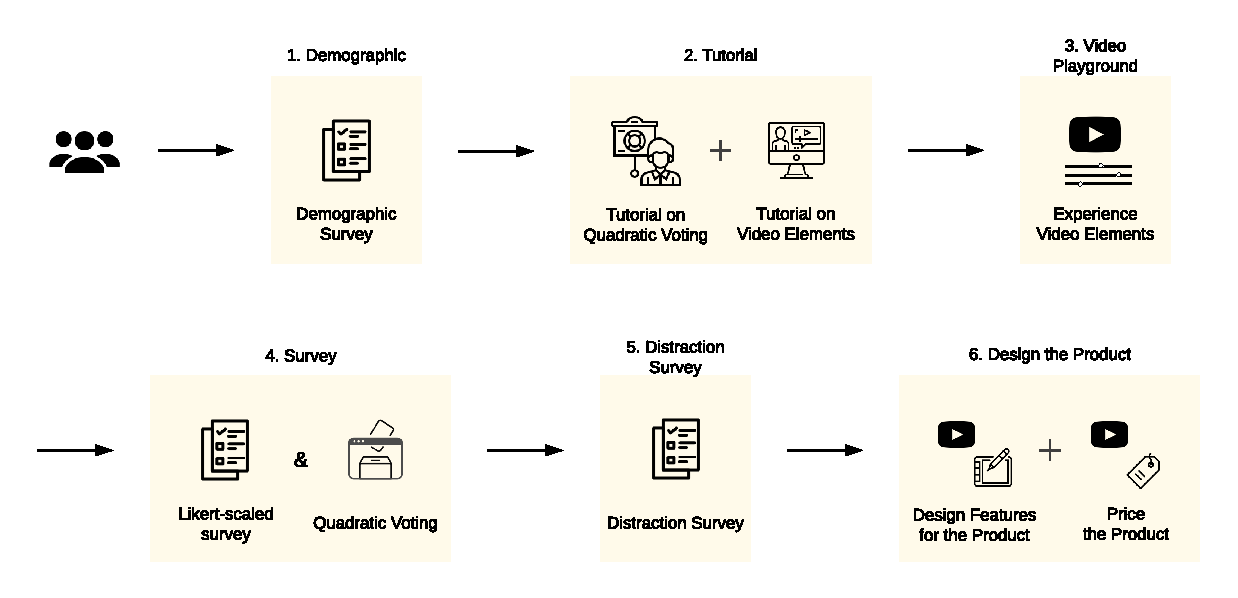
\includegraphics[width=\textwidth, keepaspectratio=true]{content/image/exp2_procedure.pdf}
    \caption{
        Experiment two is conducted within subjects. We divided participants into two groups, for which one would complete the Likert survey and then quadratic voting; the other group vice versa.
    }
    \label{fig:exp2_flow}
\end{figure}

\subsection{Experiment Flow}

To compare how well the Likert survey and QV reflect people's underlying preferences, we designed the following experiment. We recruited participants through MTurk. Like our first experiment, we use the demographic survey to make sure the participants match the U.S. demographic in age and education. All participants followed six steps, each represented in a shaded area in Figure \ref{fig:exp2_flow}. The six steps are (1) demographics survey, (2) tutorials and attention checks, (3) a video playground, (4) two surveys, (5) a distraction survey, and (6) a design task. The experiment takes about 45 minutes to complete. Turkers will receive a compensation of \$6 U.S. dollars if they complete their work and a possible bonus up to \$2 dollars. Now we explain the six steps in detail with the actual study provided as supplementary material.

\subsubsection{Step 1. Demographic}
We greeted participants with a consent form. In the consent form, we told the participants that the study aims to collect how different people think about the importance of the different elements when watching a video. We did not reveal to the participants that this experiment aimed to compare Likert and QV until they completed the survey. Once participants gave their consent, participants would fill out a demographic survey. The demographic survey contained questions identical to the first experiment.

\subsubsection{Step 2. Tutorials and attention checks}
In step two, we provided two tutorials to the participants. All participants would read through a tutorial that defined the five video elements described in the experiment. In this tutorial, for each video element, we showed a pair of videos side-by-side for participants to compare how the same video would differ if a particular element were perfect and when the element is of lousy quality. Once the participants thought they understood the concepts, we asked them to answer five multiple choice questions related to the tutorial concepts. We also included two attention checks to make sure the participant's audio and video worked fine. Participants would be disqualified from the experiment immediately if they answered two or more of the questions incorrectly. This step makes sure participants fully understand the terminology used for the rest of the experiment.

Participants would then move to the tutorial on QV since QV is unpopular among the mass. The tutorial provided a short video explaining QV supplemented with text. Participants were allowed to play with the QV interface similar to Figure \ref{fig:qv_donation} with types of cuisine as the options. Once participants are confident that they understand QV, they need to complete a quiz consisting of five true-false questions and two attention questions. The system would disqualify the participants immediately if they answered two or more of the questions incorrectly.

\begin{figure}[htpb]
    \centering
    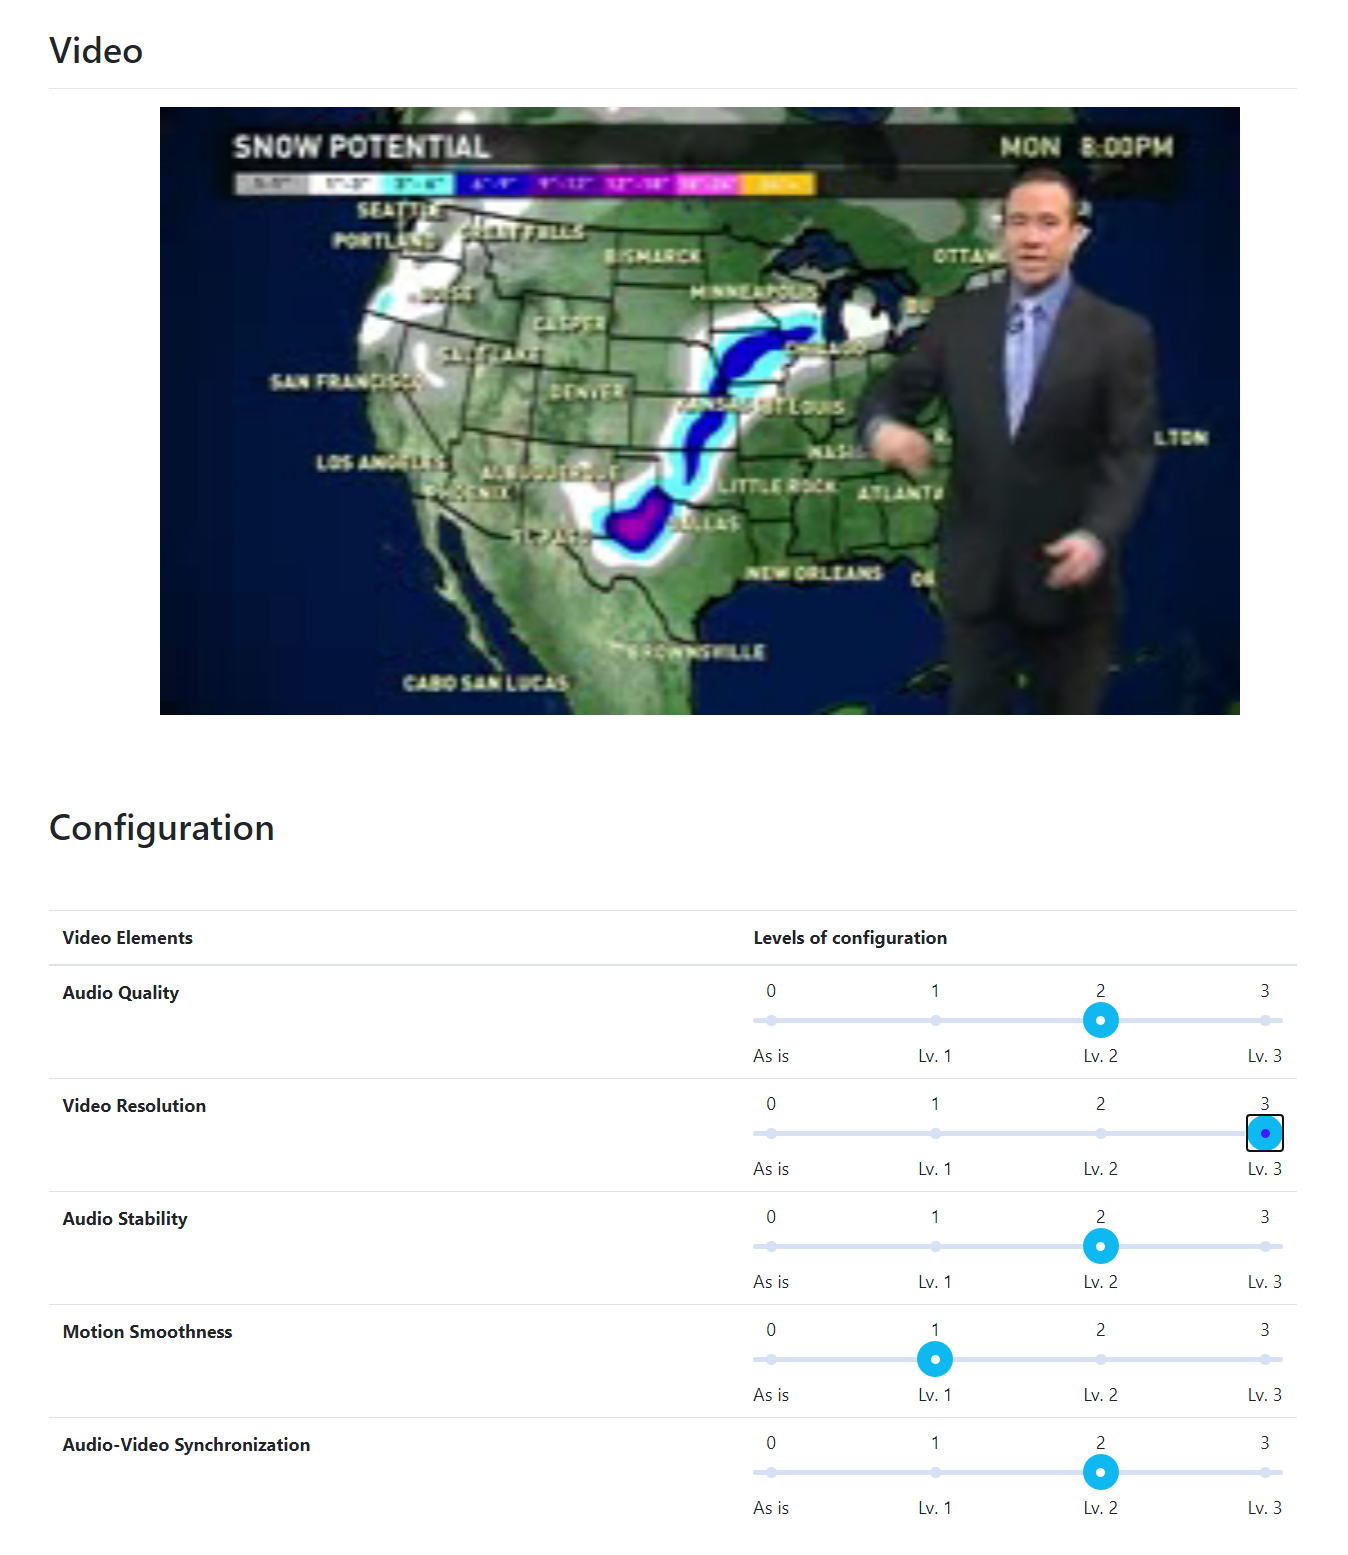
\includegraphics[width=0.8\textwidth, keepaspectratio=true]{content/image/video_playground.png}
    \caption{
        The Real-time Video Element Interface allows participants to adjust and understand how different video playback elements impact their viewing experience. We selected different levels for tech setting toggles according to prior research. The technical details of this implementation are included in the appendix.
    }
    \label{fig:exp2_playground}
\end{figure}


\subsubsection{Step 3. Video Playground}
To increase this experiment's fidelity, we introduced a fictional company to the participants, explaining that the goal is to ultimately provide a video-streaming product to the automotive industry using satellite-based internets. We first showed participants the current prototype of the company's streaming service under limited bandwidth, which was a weather forecast video with all five elements at the worst quality in the range we designed to study\footnote{Motion smoothness: 32\% packet loss rate; Audio stability: 32\% packet loss rate; Video resolution: 210x280; Audio quality: 8kHz sampling rate; Audio-video synchronization: audio plays 2250ms ahead of the video}. After experiencing the current prototype, the participants moved on to the next page.

We then instructed them to explore how various enhancement levels on different elements in the current prototype would improve their viewing experience. To help them better understand the enhancements' impact, we built a video playground shown in Fig \ref{fig:exp2_playground}. This playground showed real-time changes in the video's overall quality as the participants adjust the control panel to a specific combination of different levels of enhancements for the five video elements. It is important to note that this interface is important because we asked participants to elicit preferences among the different \textit{perspectives} of the same subject matter. Each of these perspectives might not be independent of one another.

This interface showcased a weather forecast video on the top of the page. For each of the five video playback elements, we provided a slider with four levels of tickers. Participants can toggle any of these five elements to any of the four levels at any time. According to the quality levels the participants set, the video playback will immediately apply those changes. Participants can pause and play the video at any time, and they can replay the video as many times as they like. We encouraged participants to test out different combinations freely in this playground.

With Level 0 at the lowest quality and Level 4 at the highest, we designed the intermediate levels based on prior research \cite{claypool1999effects,oeldorf2012bad, noll1993wideband,knoche2008low, steinmetz1996human} such that the changes between each level of an element have a quasi-linear impact on viewers' perception. The five levels of the five video playback elements are listed below, from Level 0 to Level 3:
\begin{itemize}
    %20\%, 8\%, 4\%, and 0\%
    \item Motion Smoothness: 32\%, 20\%, 8\%, 4\%, and 0\%
    %20\%, 8\%, 4\%, and 0\%
    \item Audio Stability: 32\%, 20\%, 8\%, 4\%, and 0\%
    %210x280, 294x392, 364x486, and 420x560     
    \item Video Resolution: 210x280, 294x392, 364x486, 420x560, and 600x800 
    %8kHz, 11kHz, 16kHz, and 48kHz 
    \item Audio Quality: 8kHz, 11kHz, 16kHz, 48kHz, and 96kHz
    %1850, 1615, 1050, or 0 ms ahead
    \item Audio-Video Synchronization: 2250ms, 1850ms,  1615ms, 1050ms, or 0ms ahead
\end{itemize}

A text box was below this interface, asking participants to describe how changing the elements impacted their experience to make sure participants did toggle the settings.

\subsubsection{Step 4. Surveying Preferences}
After the participants were confident, they understood how the enhancements on different video playback elements would impact their viewing experience and complete the short question. We collected participants' feedback on how critical the improvements on each video element in the current prototype understand the weather forecast video's content. We divided all participants into two groups: the first group would complete the Likert survey first followed by a QV survey; the second group would complete the same two surveys in reverse order. The interface for Likert and QV are provided in the supplementary materials. The QV interface is similar to Figure \ref{fig:qv_donation}, for which each of the societal causes is now the five video elements. Unlike the previous experiment, we randomized the orders of each participant's options to prevent ordering effects. Our findings from experiment one allowed us to designed the credit budget to be 100 voice credits, derived from $N^2 x O$, where $N=5$ and $O=4$.

\subsubsection{Step 5. Distraction Survey}
Before moving on to the task that elicits the participant's underlying preference, we designed a distraction survey similar to experiment one. This survey prevents participants from translating their survey responses directly to the tasks that are to follow. We also told participants that this survey results would be used in a matching process for the next task. This survey asked participants' preferences across different subscription tiers for several well-known streaming services.

\subsubsection{Step 6. Design a Product}
Participants complete the experiment by designing a product. This task aims to capture a participant's actual underlying preferences on how critical they \textit{value} each of the five video elements. This is non-trivial, especially compared to our previous design using donations. We need to design a scenario and collect the behavioral data when participants are interacting with the task. We created the ``Design a Product'' task.

To create a high fidelity scenario, we told participants that the system distributed them into the designer group, who will design and assemble a streaming service for cars via satellite internet. Their goal is to design and price their product such that another participant, similar to them based on demographic information and the distraction survey from the buyers' group, would be willing to purchase the product. We emphasized to the participants that it is important to design the product such that it is affordable but allows the buyer to understand the weather forecast video's content.

The instruction also told participants to consider that each element is associated with a cost, and the buyer will need to pay each element's cost. We told participants that if the buyer decides to purchase the product, they will receive 10\% of the final price they proposed as their commission. 

There are two steps to guide participants to complete this task. We provided the interface for the two steps in Figure \ref{fig:exp2_store}. The first step starts by asking participants to select one of the two quality for each video element and ``assemble'' the product. In the second step, participants were asked to provide a price they think are reasonable to the five elements based on the qualities they selected. The sum of these price tags becomes the total price of the product. Participants were reminded throughout this task that the higher they priced the elements, the more their bonus could be. However, if they price the product too high, buyers might not purchase their design, and they would fail to gain any bonuses. 

Participants do not know that there does not exist a ``buyers'' group in this task. The goal of this design is to figure out the willingness-to-pay for each participant. One could view this task as a reverse auction, in which participants need to price how they value each of the elements according to their beliefs. If they price the product higher than their accurate valuations, this means that the ``buyer'' that is similar to them would reject their proposal, given the likely value the elements the same. Vice versa, if the participants set their prices lower than their belief, they lose out on potential opportunities to earn the bonuses. This made this task incentive-compatible. 

\begin{figure}[htpb]
    \centering
    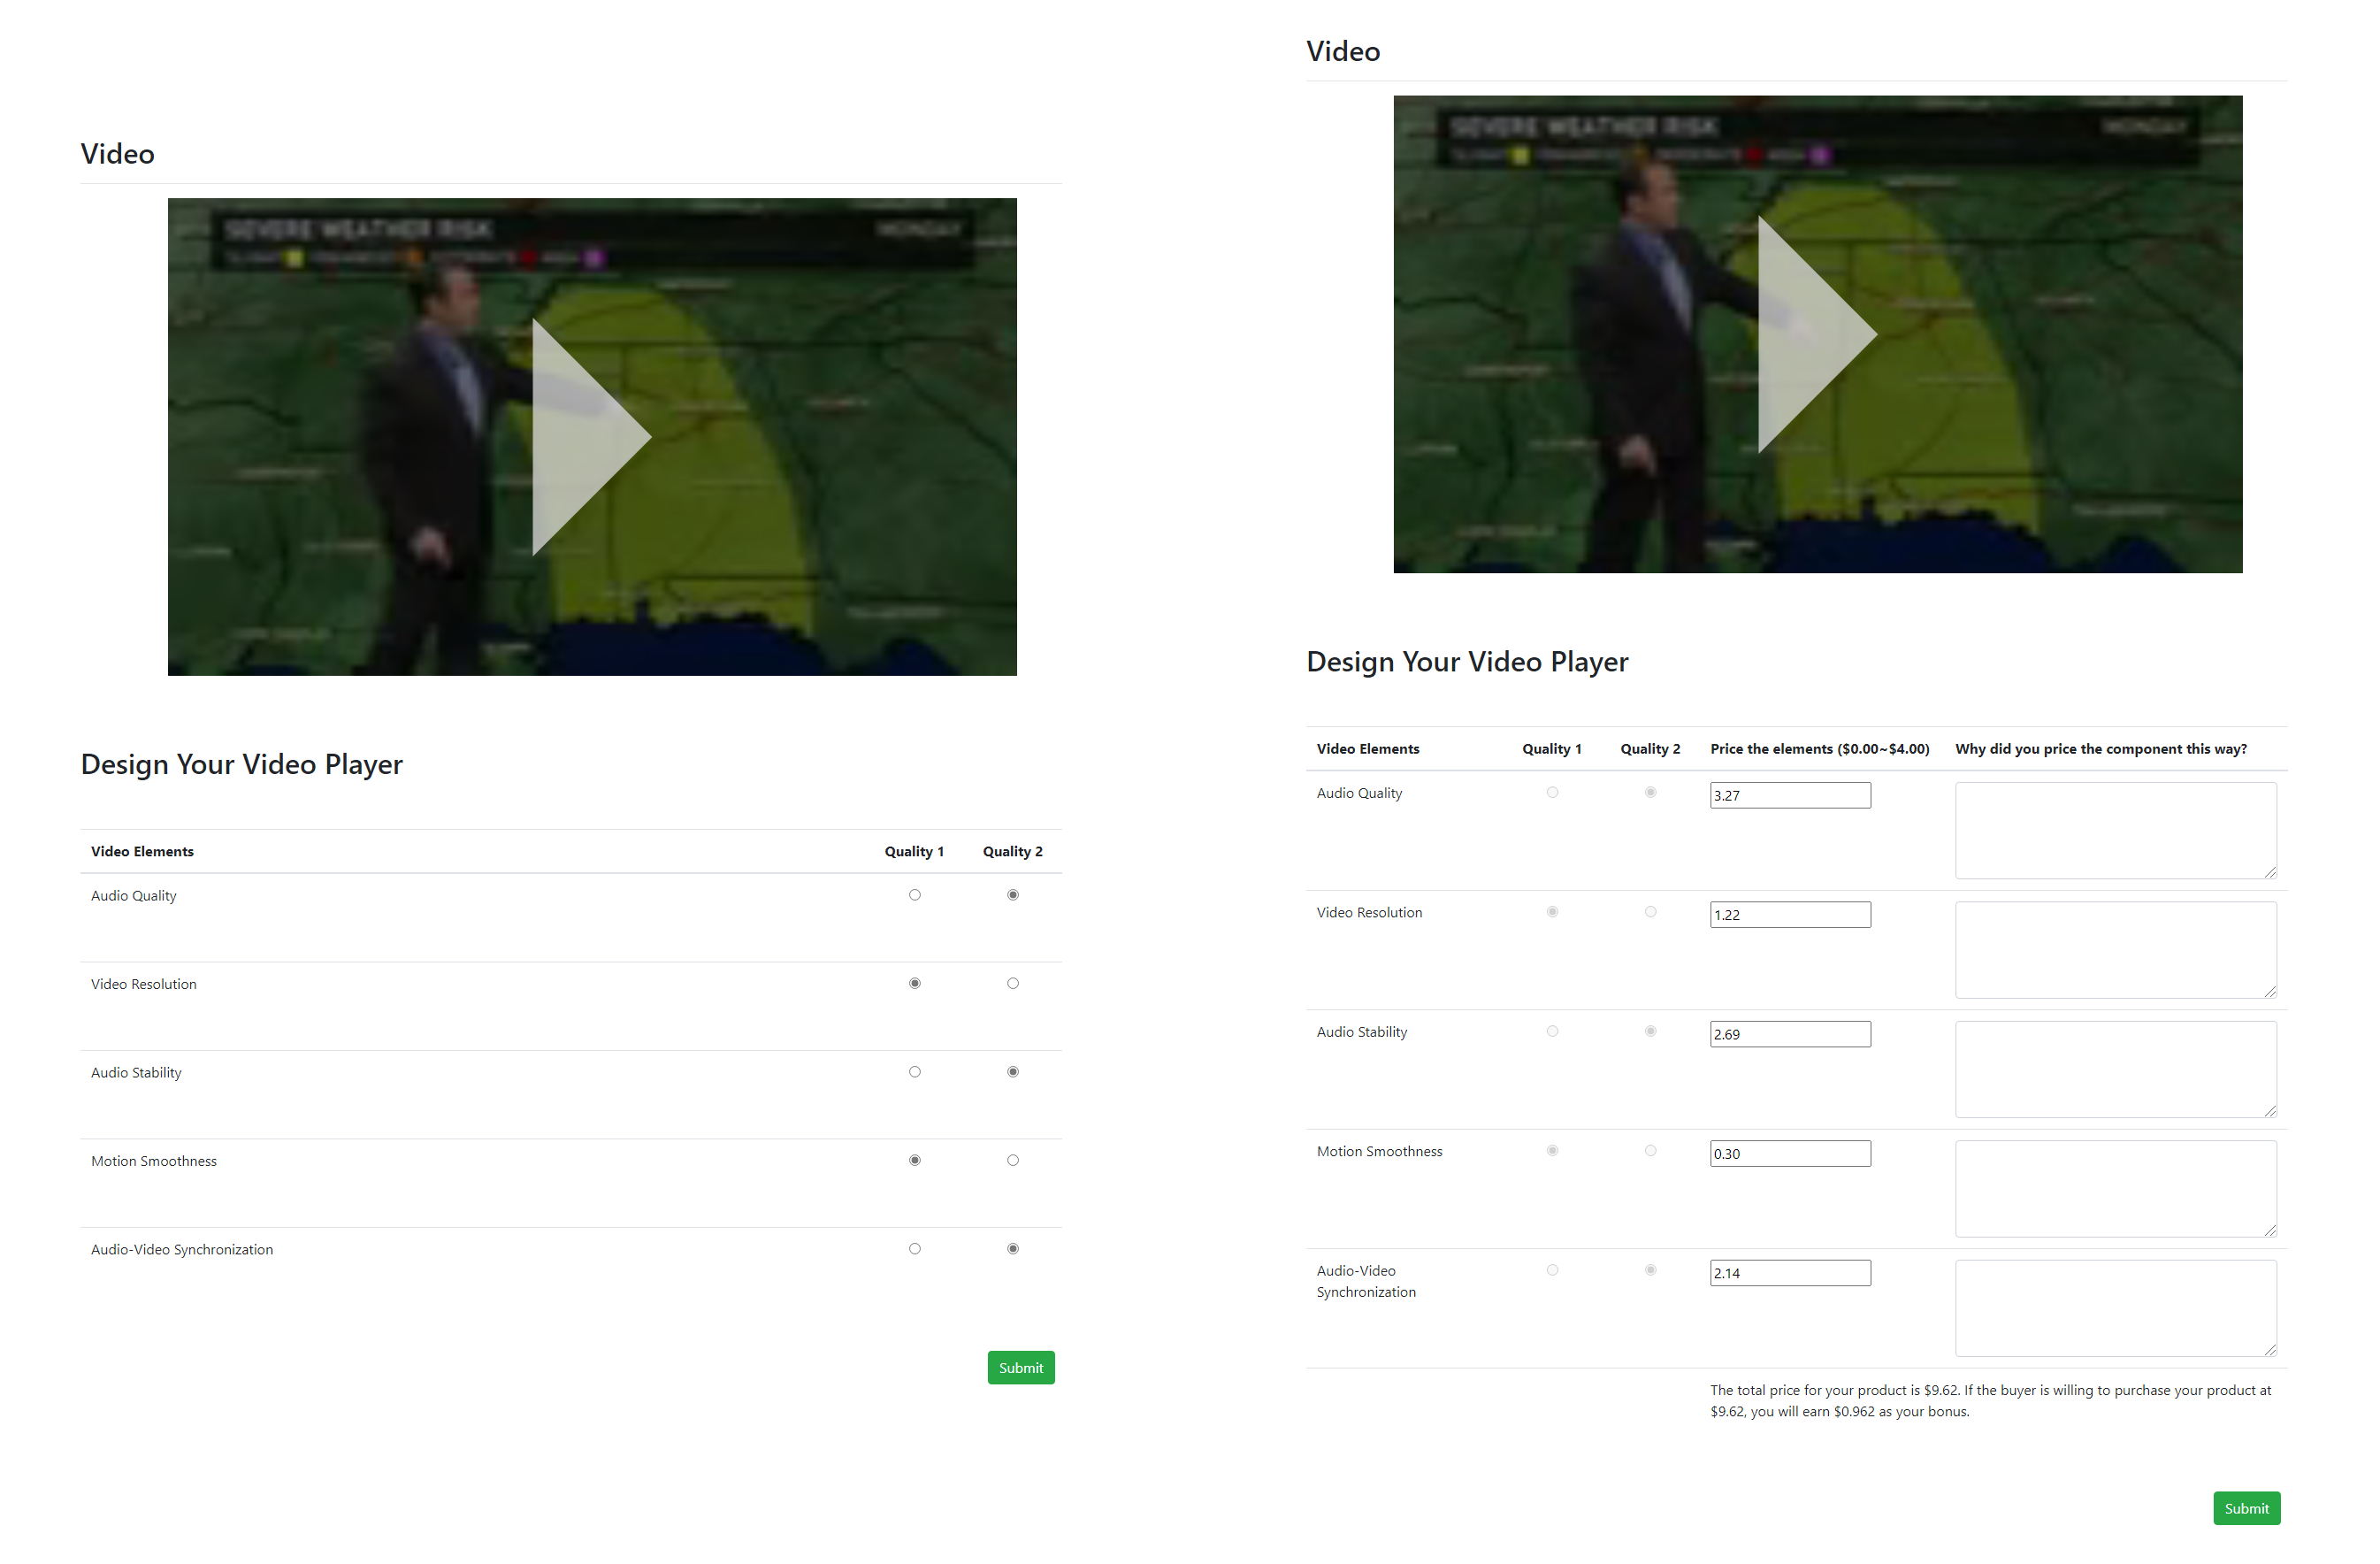
\includegraphics[width=\textwidth, keepaspectratio=true]{content/image/design_task.png}
    \caption{
        The two steps participants encounter when completing Step 6 of the survey. Participants would first need to elect the quality that they would involve into their video streaming product. Participants can see real time changes to the video as they select the combinations. Once they made their decision, participants would price each of the elements, each of them up to \$4 dollars. Participants would recieve a commission of 2\% based on some criteria.
    }
    \label{fig:exp2_store}
\end{figure}

Notice that instead of giving participants the power to select the quality over various levels as they did in the video playground in step three. We only provide two qualities for each video element. Quality one refers to level 0 in the playground, basically the worst one they had experienced. However, for quality 2, we designed the values to match prior research claiming that quality is the ``accepted level'' in their experiment\footnote{Place the five quality two values here}. This binary design prevents us from bounding participants' choices when provided a slider. Participants are essentially making a decision of whether a video element is ``important'' or ``not important.''

\subsection{System Design}
In this experiment, we build on top of the system for experiment one. To create real-time adjustments, we created the different qualities of video and audio files independently ahead of the experiment. When there is a change in the audio or video quality toggle, the system serves the correct combinations of video and audio files. JavaScript in the front-end was responsible for creating the video-audio synchronization and video/audio packet loss effects.
This design balances the need for network speed, preventing from streaming every configuration from the server. It also prevents the need for a powerful client such that video and audio qualities were not computed directly on the client. The experiment source code for experiment two is publicly available \footnote{Not yet public}, and so is the video interface as a stand-alone repository \footnote{https://github.com/hank0982/QV-app}. More details are provided in the appendix.